\documentclass[12pt]{extarticle}
%Some packages I commonly use.
\usepackage[portuguese]{babel}
\usepackage{graphicx}
\usepackage{framed}
\usepackage[normalem]{ulem}
\usepackage{amsmath}
\usepackage{amsthm}
\usepackage{amssymb}
\usepackage{amsfonts}
\usepackage{enumerate}
\usepackage[utf8]{inputenc}
\usepackage{float}
\usepackage{gensymb}
\usepackage[top=1 in,bottom=1in, left=1 in, right=1 in]{geometry}
\usepackage{multirow}
\usepackage{caption}
\usepackage{subcaption}
\usepackage[utf8]{inputenc}

%A bunch of definitions that make my life easier
\newcommand{\matlab}{{\sc Matlab} }
\newcommand{\cvec}[1]{{\mathbf #1}}
\newcommand{\rvec}[1]{\vec{\mathbf #1}}
\newcommand{\ihat}{\hat{\textbf{\i}}}
\newcommand{\jhat}{\hat{\textbf{\j}}}
\newcommand{\khat}{\hat{\textbf{k}}}
\newcommand{\minor}{{\rm minor}}
\newcommand{\trace}{{\rm trace}}
\newcommand{\spn}{{\rm Span}}
\newcommand{\rem}{{\rm rem}}
\newcommand{\ran}{{\rm range}}
\newcommand{\range}{{\rm range}}
\newcommand{\mdiv}{{\rm div}}
\newcommand{\proj}{{\rm proj}}
\newcommand{\R}{\mathbb{R}}
\newcommand{\N}{\mathbb{N}}
\newcommand{\Q}{\mathbb{Q}}
\newcommand{\Z}{\mathbb{Z}}
\newcommand{\<}{\langle}
\renewcommand{\>}{\rangle}
\renewcommand{\emptyset}{\varnothing}
\newcommand{\attn}[1]{\textbf{#1}}
\theoremstyle{definition}
\newtheorem{theorem}{Theorem}
\newtheorem{corollary}{Corollary}
\newtheorem*{definition}{Definition}
\newtheorem*{example}{Example}
\newtheorem*{note}{Note}
\newtheorem{exercise}{Exercise}
\newcommand{\bproof}{\bigskip {\bf Proof. }}
\newcommand{\eproof}{\hfill\qedsymbol}
\newcommand{\Disp}{\displaystyle}
\newcommand{\qe}{\hfill\(\bigtriangledown\)}
\setlength{\columnseprule}{1 pt}
\usepackage[utf8]{inputenc}

\title{Aula 11 - Energia Elestrostática e Potencial Elétrico}
\author{Felipe Salvador}
\date{Atualizado em \today}

\begin{document}

\maketitle

\section{Introdução - Intuição}

Nessa aula, começaremos a tratar de uma formulação um pouco mais completa sobre a eletricidade, usando o princípio mais fundamental de toda a Física: \textbf{A conservação de Energia}.

\textbf{Energia é um conceito físico para quantificar o quanto um objeto está em movimento (energia cinética), o quão quente ele está (energia térmica) ou o quanto esse objeto pode mudar o sistema a qual ele está inserido (energia potencial).} O último caso depende de que interação estamos tratando, como a gravidade ou força elétrica. \textbf{Esse princípio e essa definição são a pedra fundamental da física.} Sem eles, nenhuma teoria que temos hoje funciona de forma apropriada ou consistente. 

Com isso, iremos colocar o assunto de eletricidade sobre a visão da energia, para conseguirmos entender melhor como funciona a eletricidade e quais quantidades estão envolvidas diretamente nesse fenômeno. No caso da eletricidade, são 2 quantidades de interesse: \textbf{A energia potencial elétrica ($U_{el}$) e o Potencial elétrico ($V$)}.

\textbf{A energia potencial elétrica traz a ideia de quantificar a interação de 2 cargas elétricas no espaço.} Isso nos dá a ideia de o quão atrativa/repulsiva 2 cargas são entre si e consequentemente, ajuda a indicar o quanto de energia pode ser gasta para fazer a atração/repulsão das partículas. Nesse caso, a energia iria ser gasta para colocar as cargas em movimento (que no fundo seria uma conversão de energia potencial elétrica em energia cinética.)

Nós sabemos pela força descrita pela Lei de Coulomb, que a força elétrica depende da distância entre as 2 cargas interagentes, além dos seus valores de carga. Quanto maior a distância, menor a força que uma carga aplica na outra, ou seja, menor a força de repulsão/atração. Ao mesmo tempo, se os valores das cargas forem maiores nominalmente (só os números, sem os sinais), a força fica maior, logo a força de atração/repulsão também fica maior.

Como estamos construindo o conceito de Energia Potencial Elétrica para que ela quantifique essa interação de atração/repulsão, então a formulação da Energia também tem que prever que a atração/repulsão é menor conforme a distância entre as cargas fica maior e que quanto maior os valores nominais das cargas, maior é a atração/repulsão de uma carga.

As mesmas discussões feitas no caso sobre o Campo Elétrico são feitas também quando estamos na ótica da energia.
\begin{itemize}
    \item Será que é possível extrair boa parte das informações quando colocamos 1 carga somente?
    \item Será que é possível mapear o comportamento da Energia Potencial no espaço quando temos somente 1 carga?
    \item Há a possibilidade de definir uma quantidade que quantifica o quanto a atração/repulsão 1 carga pode gerar?
\end{itemize}

A resposta de todas essas questões é \textbf{SIM}. E isso é possível, fazendo a definição do \textbf{Potencial Elétrico} (lembrando que não é Energia Potencial Elétrica, é Potencial Elétrico somente). Essa quantidade fará o mapeamento do comportamento da Energia Potencial Elétrica, qualitativamente nos dirá sobre a atração/repulsão e dar a ideia sobre o quão grande é essa energia em relação à distância.

\section{Formulação}

A Energia Potencial Elétrica $U_{el}$ é descrita como:
\begin{equation}
    \boxed{U_{el} = \frac{K_0\,q_1\,q_2}{d}}
\end{equation}
\noindent em que $K_0$ é a constante eletrostática, $q_1,\,q_2$ são as cargas envolvidas e $d$ é a distância entre as cargas. Lembrando que $d= \sqrt{(x_1-x_2)^2+(y_1-y_2)^2}$, em que $(x_1,y_1)$ é a posição da carga 1 e $(x_2,y_2)$ é a posição da carga 2.

Para encontrar o potencial elétrico, basta separar a segunda carga da fórmula:
\begin{equation}
    U_{eq} = \frac{K_0\,q_1}{d}q_2
\end{equation}

A fração é o que chamamos de \textbf{Potencial Elétrico}:
\begin{equation}
    \boxed{V = \frac{K_0\,q_1}{d}}
\end{equation}

Com isso, podemos relacionar a Energia Potencial Elétrica com o Potencial elétrico da seguinte forma:
\begin{equation}\label{eq:4}
    \boxed{U_{el}=q\,V}
\end{equation}

A unidade de $U_{el}$ é a unidade de energia: Joule - J, já a unidade de $V$ é chamada de Volt (V). Ao analisar a fórmula, percebemos que ela tem uma similaridade com a fórmula do campo elétrico:
\begin{equation}
    E=\frac{K_0\,q_1}{d^2}
\end{equation}

A diferença entre essas 2 fórmulas é que a fórmula do campo elétrico tem um fator 1/d a mais, com isso:
\begin{equation}
    E = \frac{K_0\,q_1}{d\,d} = \frac{1}{d}.\frac{K_0\,q_1}{d} = \frac{V}{d}
\end{equation}
Com isso, temos a relação do potencial elétrico com o campo elétrico:
\begin{equation}
    \boxed{V = E\,d}
\end{equation}

\textbf{Essa relação só é válida para campos elétricos uniformes e não-nulos.}

Outra relação entre o potencial e o campo elétrico é que \textbf{a direção e sentido do campo elétrico sempre vai do lugar de potencial maior para o lugar de menor potencial}, lembrando que, aqui, é de forma geral. 

Ou seja, se um lugar tiver um potencial -10 V e outro lugar com um potencial de -5 V, a flecha do campo elétrico começa no lugar com -5V e aponta para o lugar com -10V, pois $-5 > -10$.

Outra questão é sobre o trabalho feito por uma força elétrica. \textbf{Trabalho é uma grandeza que mede a conversão de um tipo de energia para outro tipo.} Normalmente, é dado ou pela letra $\tau$ ou por W. O trabalho que uma força elétrica faz é:

\begin{equation}
    \tau = q(V_f - V_i) = q\Delta V
\end{equation}
\noindent em que 'q' é a carga que está se movendo e que a força elétrica está sendo aplicada e $V_i$ e $V_f$ são os valores do potencial elétrico no lugar de início e de fim do movimento, respectivamente.
\subsection{Propriedades}

Assim como o campo elétrico, podemos determinar o comportamento da energia potencial elétrica num espaço com diversas cargas. Para determinar a energia potencial que uma carga dessas cargas terá, vamos supor um sistemas com 3 cargas, como a figura a seguir:
\begin{figure}[H]
    \centering
    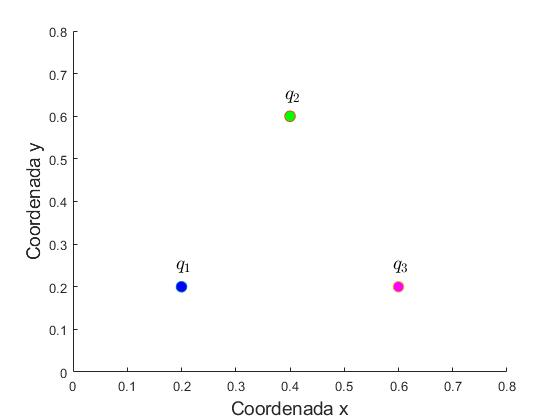
\includegraphics[width=0.8\textwidth]{ex_1.jpg}
    \caption{Um sistema de 3 cargas}
    \label{fig:ex_1}
\end{figure}

A energia potencial total que a carga 2 irá sentir será a soma da energia potencial que a carga 2 interage com a carga 1 e que a carga 2 interage com a carga 3. Por isso:
\begin{equation}
\begin{split}
    U_2 &= U_{12} + U_{32} = \frac{K_0\,q_1\,q_2}{d_{12}} + \frac{K_0\,q_3\,q_2}{d_{32}} = q_2\left(\frac{K_0\,q_1}{d_{12}} + \frac{K_0\,q_3}{d_{32}}\right) = (V_{12} +V_{32})q_2\\
    U_2 &=(V_{12} +V_{32})q_2
    \end{split}
\end{equation}
\noindent em que $V_{12}$ é o Potencial Elétrico da carga 1 calculado na posição da carga 2 e $V_{32}$é o Potencial Elétrico da carga 3 calculado na posição da carga 2. Pela fórmula (\ref{eq:4}), a expressão do parêntesis é o potencial elétrico total, calculado na posição da carga 2:
\begin{equation}
    V_2 = V_{12} +V_{32}
\end{equation}

\textbf{De forma geral, a energia potencial que uma carga sente é o produto da carga com a soma dos potenciais elétricos gerados pelas outras cargas, calculados na posição da carga de interesse.}:
\begin{equation}
    U_2 = (V_{12} + V_{32} + V_{42} + V_{52} + \dots)q_2
\end{equation}

Com o potencial elétrico, podemos mapear o comportamento da energia no espaço. E para ilustrar melhor isso, podemos fazer um gráfico que desenha linhas tal que, sobre uma linha, a energia tem um valor definido:
\begin{figure}[H]
    \centering
    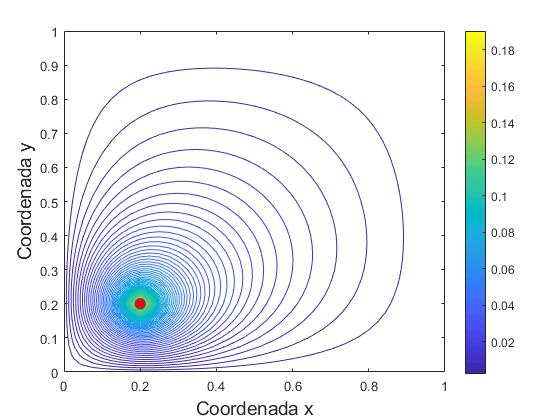
\includegraphics[width=0.7\textwidth]{potential_1.jpg}
    \caption{Gráfico das linhas equipotenciais - sobre cada linha, o valor do Potencial Elétrico (V) é constante. A cor da linha tem um significado em relação ao valor do potencial e colocamos essa barra de cor para fazer a relação. O ponto vermelho é a carga elétrica. Nesse caso, é o potencial gerado por uma carga pontual.}
    \label{fig:potential_point}
\end{figure}

Como acima, podemos fazer um sistema com inúmeras cargas envolvidas. Um caso de interesse é quando queremos analisar o potencial de um par de cargas, em que uma é positiva e a outra é negativa. Chamamos esse par de \textbf{dipolo}:
\begin{figure}[H]
    \centering
    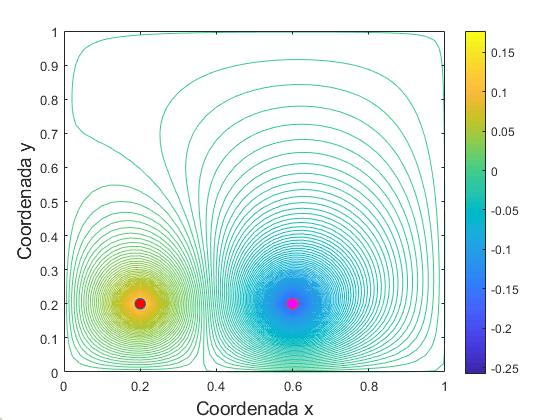
\includegraphics[width=0.8\textwidth]{potential_dipole.jpg}
    \caption{Gráfico das linhas equipotenciais de um potencial elétrico feito por um dipolo. Em vermelho, está a carga positiva, enquanto em rosa está a carga negativa.}
    \label{fig:potential_dipole}
\end{figure}

Se o trabalho sobre uma carga for feito de forma que o ponto inicial e final estiverem sobre uma mesma linha equipotencial, ou seja, os pontos possuem um mesmo valor de potencial elétrico, então:
\begin{equation}
    \tau=q(V-V) = q\,0 = 0
\end{equation}
\noindent ou seja, o trabalho feito sobre uma carga que começou e terminou sobre uma linha equipotencial é nulo.
\begin{figure}[H]
    \centering
    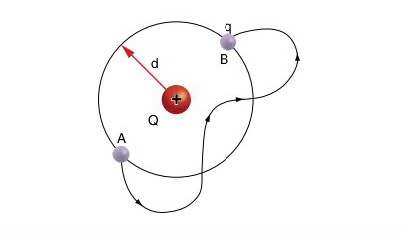
\includegraphics[width=0.6\textwidth]{equipotencial_work.png}
    \caption{Exemplo esquemático de uma carga que sofre um trabalho nulo. Os pontos inicial e final do trabalho estão sobre uma mesma equipotencial.}
    \label{fig:work_equipotential}
\end{figure}
\section{Potencial elétrico e condutores}

\textbf{Vimos na aula passada que o campo elétrico dentro de um condutor é sempre zero.} Bem, isso se relaciona com o potencial elétrico da seguinte forma:

\textbf{O potencial elétrico dentro de um condutor é sempre constante, podendo ser 0, por exemplo.}

Um condutor quando é aterrado, ou seja, ligado à Terra, o potencial elétrico desse condutor é 0.
\begin{figure}[H]
    \centering
    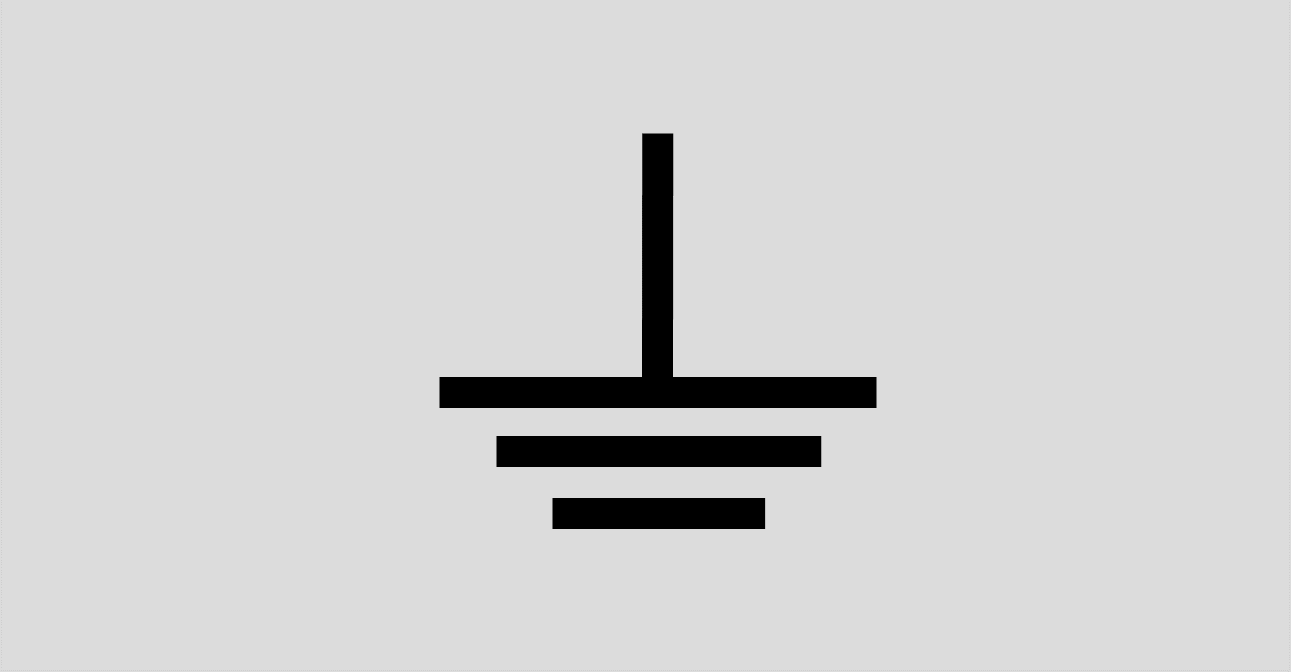
\includegraphics[width=0.2\textwidth]{Introducao-sobre-os-tipos-de-aterramento.png}
    \caption{Símbolo de aterramento. Quando algum objeto tem um fio em que numa ponta tem esse símbolo, significa que o objeto está aterrado, ou seja, que o potencial elétrico dele é 0.}
    \label{fig:my_label}
\end{figure}
\end{document}
